% !TeX program = xelatex
\documentclass[a4paper,10pt]{article}

% ============================================================================
% សន្លឹកកិច្ចការសិស្ស ស-ខ្មៅ (Student Fill-In Worksheet — No-LCD Classroom)
% មេរៀនទី១៦ (១៦.៤.១)៖ កន្លះបន្ទាត់ពុះមុំក្នុងនៃត្រីកោណ (ត្រូវគ្នា ១០០% នឹង LS_Plan_INB.tex)
% ============================================================================
\usepackage[a4paper, left=0.95cm, right=0.95cm, top=0.75cm, bottom=0.90cm, footskip=0.48cm]{geometry}
\usepackage{amsmath}
\usepackage{unicode-math}
\usepackage{fontspec}
\usepackage{array, colortbl}
\usepackage[table]{xcolor}
\usepackage{enumitem}
\usepackage{pifont}
\usepackage{fancyhdr}
\usepackage{lastpage}
\usepackage{tikz}
\usepackage[most]{tcolorbox}
\usetikzlibrary{calc, arrows.meta, angles, quotes, decorations.markings, babel}

\makeatletter
\let\@expl@@@mark@update@singlecol@structures@@\relax
\makeatother

% ============================================================================
% ការកំណត់ពុម្ពអក្សរ (Cross-Platform Font Resolver)
% ============================================================================
\providecommand{\NGSFindFonts}{%
  \IfFileExists{C:/Windows/Fonts/cambria.ttc}{%
    \def\NGSSysPath{C:/Windows/Fonts/}%
    \def\NGSUserPath{C:/Users/KIT/AppData/Local/Microsoft/Windows/Fonts/}%
  }{%
    \IfFileExists{./fonts/KhmerOSsiemreap.ttf}{\def\NGSSysPath{./fonts/}\def\NGSUserPath{./fonts/}}{%
    \IfFileExists{../fonts/KhmerOSsiemreap.ttf}{\def\NGSSysPath{../fonts/}\def\NGSUserPath{../fonts/}}{%
    \IfFileExists{../../fonts/KhmerOSsiemreap.ttf}{\def\NGSSysPath{../../fonts/}\def\NGSUserPath{../../fonts/}}{%
    \IfFileExists{../../../fonts/KhmerOSsiemreap.ttf}{\def\NGSSysPath{../../../fonts/}\def\NGSUserPath{../../../fonts/}}{%
    \IfFileExists{../../../../fonts/KhmerOSsiemreap.ttf}{\def\NGSSysPath{../../../../fonts/}\def\NGSUserPath{../../../../fonts/}}{%
    \IfFileExists{../../../../../fonts/KhmerOSsiemreap.ttf}{\def\NGSSysPath{../../../../../fonts/}\def\NGSUserPath{../../../../../fonts/}}{%
    \IfFileExists{../../../../../../fonts/KhmerOSsiemreap.ttf}{\def\NGSSysPath{../../../../../../fonts/}\def\NGSUserPath{../../../../../../fonts/}}{%
      \def\NGSSysPath{../../../../../../../fonts/}\def\NGSUserPath{../../../../../../../fonts/}%
    }}}}}}}%
  }%
}
\NGSFindFonts

\setmathfont[Path={\NGSSysPath}, FontIndex=1, Scale=1.02]{cambria.ttc}
\defaultfontfeatures{Ligatures=TeX}

\setmainfont[
  Path={\NGSUserPath},
  Extension=.ttf,
  Script=Khmer,
  BoldFont={KhmerOSsiemreap},
  BoldFeatures={FakeBold=1.8},
  ItalicFont={KhmerOSsiemreap},
  ItalicFeatures={FakeSlant=0.25},
  BoldItalicFont={KhmerOSsiemreap},
  BoldItalicFeatures={FakeBold=1.8, FakeSlant=0.25}
]{KhmerOSsiemreap}

\newfontfamily\muol[Path={\NGSUserPath}, Extension=.ttf, Script=Khmer]{KhmerOSmuollight}
\newfontfamily\TimesEn[Path={\NGSSysPath}, Extension=.ttf, BoldFont={timesbd}, ItalicFont={timesi}, BoldItalicFont={timesbi}]{times}

\XeTeXlinebreaklocale "km"
\XeTeXlinebreakskip = 0pt plus 1pt minus 0.1pt

\definecolor{panelgray}{gray}{0.93}
\definecolor{headgray}{gray}{0.85}

\pagestyle{fancy}
\fancyhf{}
\renewcommand{\headrulewidth}{0pt}
\fancyfoot[L]{\fontsize{8pt}{10pt}\selectfont អនុវិទ្យាល័យព្រះក្រសាំង \en{---} គណិតវិទ្យា ថ្នាក់ទី៨ \en{|} មេរៀនទី១៦ (១៦.៤ កន្លះបន្ទាត់ពុះមុំក្នុងនៃត្រីកោណ)}
\fancyfoot[R]{\fontsize{8.2pt}{10pt}\selectfont ទំព័រ \en{\thepage\ / \pageref{LastPage}}}

\setlength{\parindent}{0pt}
\setlength{\parskip}{0pt}
\setlength{\tabcolsep}{4pt}

\newcommand{\en}[1]{{\TimesEn #1}}
\newcommand{\enbf}[1]{{\TimesEn\textbf{#1}}}
\newcommand{\unit}[1]{\,\text{\en{#1}}}
\newcommand{\cnum}[1]{\mbox{\fontsize{10pt}{12pt}\selectfont\ding{\numexpr181+#1\relax}}}
\newcommand{\chkbox}{\tikz[baseline=-0.15ex]\draw[black, line width=0.85pt] (0,0) rectangle (0.25cm,0.25cm);}
\newcommand{\blank}[1]{\makebox[#1]{\dotfill}}
\newcommand{\tri}[1]{\ensuremath{\triangle #1}}
\newcommand{\ang}[1]{\ensuremath{\angle #1}}
\newcommand{\cg}{\ensuremath{\cong}}

\newcommand{\rightbox}[4][0.18]{%
  \draw[black, line width=0.8pt]
    ($(#3)!#1!(#2)$) -- ($($(#3)!#1!(#2)$)+($(#3)!#1!(#4)$)-(#3)$) -- ($(#3)!#1!(#4)$);
}

\newcommand{\secbar}[2]{%
  \vspace{3pt}%
  \begin{tcolorbox}[
    enhanced, sharp corners, colback=headgray, colframe=black,
    boxrule=0.9pt, boxsep=1pt, top=2.5pt, bottom=2.5pt, left=6pt, right=6pt,
    after skip=3pt
  ]
    {\muol\fontsize{9.2pt}{13.5pt}\selectfont #1}\hfill{\fontsize{8.3pt}{11.5pt}\selectfont\textbf{#2}}
  \end{tcolorbox}%
}

\tikzset{
  tk1/.style={postaction={decorate},decoration={markings,mark=at position 0.50 with {\draw[black, line width=0.90pt](0,-0.095)--(0,0.095);}}},
  tk2/.style={postaction={decorate},decoration={markings,
    mark=at position 0.45 with {\draw[black, line width=0.90pt](0,-0.095)--(0,0.095);},
    mark=at position 0.55 with {\draw[black, line width=0.90pt](0,-0.095)--(0,0.095);}}}
}

\newcolumntype{L}[1]{>{\raggedright\arraybackslash}p{#1}}
\newcolumntype{C}[1]{>{\centering\arraybackslash}p{#1}}

\begin{document}
\fontsize{9.4pt}{13.8pt}\selectfont

% ============================================================================
% ទំព័រទី ១៖ ក្បាលសន្លឹកកិច្ចការ + E1 + E2 (ពិសោធកាំកែង vs អង្កត់ទ្រេត & សម្រាយបំភ្លឺ) + E3
% ============================================================================
\begin{tcolorbox}[
  enhanced, sharp corners, colback=white, colframe=black,
  boxrule=1.1pt, boxsep=2pt, top=4pt, bottom=4pt, left=6pt, right=6pt, after skip=5pt
]
  \begin{center}
    {\muol\fontsize{10.2pt}{14.8pt}\selectfont សន្លឹកកិច្ចការសិស្ស \enbf{---} គណិតវិទ្យា ថ្នាក់ទី៨ \enbf{(}១៦\enbf{.}៤ កន្លះបន្ទាត់ពុះមុំក្នុងនៃត្រីកោណ\enbf{)}}\\[2pt]
    {\fontsize{8.8pt}{12pt}\selectfont
    ឈ្មោះសិស្ស / ដៃគូ៖ \blank{6.2cm} \hspace{0.2cm}
    ថ្នាក់៖ \blank{1.4cm} \hspace{0.2cm}
    ក្រុម៖ \blank{1.2cm} \hspace{0.2cm}
    កាលបរិច្ឆេទ៖ \blank{2.8cm}}
  \end{center}
\end{tcolorbox}

% --- E1 Engage ---
\begin{tcolorbox}[
  enhanced, sharp corners, colback=panelgray, colframe=black,
  boxrule=0.8pt, boxsep=2pt, top=4pt, bottom=4pt, left=6pt, right=6pt, after skip=5pt
]
  \textbf{បេសកកម្មទី១ (\en{E1 - Engage})៖ អាងឈូករាងរង្វង់ធំបំផុតប៉ះផ្លូវដើរទាំងបីនៃសួនត្រីកោណ $\tri{ABC}$}\\
  សាលាចង់សង់អាងឈូករាងរង្វង់ក្នុងសួនត្រីកោណ $\tri{ABC}$ ឱ្យប៉ះផ្លូវដើរទាំងបី $AB, BC, CA$ ស្មើគ្នា ។ ចូរទស្សន៍ទាយមុនពិសោធន៍៖\\
  $\blacktriangleright$ (១) ផ្ចិតអាងគឺ៖ \chkbox\ ផ្ចិត $O$ (ប្រសព្វមេដ្យាទ័រ) \hspace{0.15cm} \chkbox\ ផ្ចិត $I$ (ប្រសព្វកន្លះបន្ទាត់ពុះមុំក្នុង) \hspace{0.2cm}
  (២) កាំរង្វង់៖ \chkbox\ អង្កត់កែង $IP$ \hspace{0.15cm} \chkbox\ អង្កត់ទ្រេត $IB'$
\end{tcolorbox}

% --- E2 Explore Part A: Tangent-Foot Contrast Lab ---
\secbar{ផ្នែកទី១ \enbf{(}ក\enbf{)} ៖ ពិសោធន៍ផ្ទៀងផ្ទាត់ផ្ចិត $I$ និងអន្ទាក់កាំរង្វង់ចារឹកក្នុង \enbf{(Tangent-Foot Lab --- E2)}}{ការងារជាដៃគូ \en{6 min}}

\noindent
\begin{minipage}[c]{8.9cm}
  \centering
  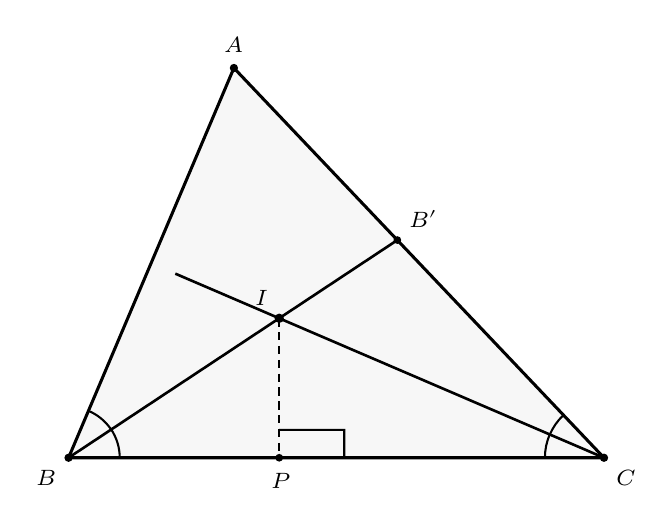
\begin{tikzpicture}[x=1cm, y=1cm, every node/.style={font=\footnotesize, text=black}]
    \coordinate (B) at (0,0);
    \coordinate (C) at (6.8,0);
    \coordinate (A) at (2.1,4.95);
    \pgfmathsetmacro{\la}{6.8}
    \pgfmathsetmacro{\lb}{veclen(4.7,4.95)}
    \pgfmathsetmacro{\lc}{veclen(2.1,4.95)}
    \pgfmathsetmacro{\per}{\la+\lb+\lc}
    \pgfmathsetmacro{\ix}{(\la*2.1+\lb*0+\lc*6.8)/\per}
    \pgfmathsetmacro{\iy}{(\la*4.95)/\per}
    \coordinate (I) at (\ix,\iy);
    \coordinate (P) at (\ix,0);
    \coordinate (Bp) at (intersection of B--I and A--C);

    \fill[gray!6] (A) -- (B) -- (C) -- cycle;
    \draw[black, line width=1.1pt] (A) -- (B) -- (C) -- cycle;
    \draw[black, line width=0.95pt] (B) -- (Bp);
    \draw[black, line width=0.95pt] (C) -- ($(C)!1.32!(I)$);
    \draw[black, line width=0.8pt, densely dashed] (I) -- (P);
    \rightbox[0.20]{I}{P}{C}

    \draw[black, line width=0.75pt] (0.65,0) arc (0:34:0.65);
    \draw[black, line width=0.75pt] (0.54,0.36) arc (34:68:0.65);
    \draw[black, line width=0.75pt] (6.05,0) arc (180:157:0.75);
    \draw[black, line width=0.75pt] (6.11,0.29) arc (157:134:0.75);

    \fill[black] (A) circle (1.5pt) node[above=2pt] {$A$};
    \fill[black] (B) circle (1.5pt) node[below left=1pt] {$B$};
    \fill[black] (C) circle (1.5pt) node[below right=1pt] {$C$};
    \fill[black] (I) circle (1.7pt) node[above left=1pt] {$I$};
    \fill[black] (P) circle (1.4pt) node[below=2pt] {$P$};
    \fill[black] (Bp) circle (1.4pt) node[above right=1pt] {$B'$};
  \end{tikzpicture}
\end{minipage}%
\hfill
\begin{minipage}[c]{9.7cm}
  \textbf{ជំហានពិសោធន៍ជាដៃគូលើរូបខាងឆ្វេង៖}\\[5pt]
  $1.$ គូសភ្ជាប់កន្លះបន្ទាត់ $AI$ រួចយករ៉ាប់ព័រទ័រវាស់ផ្ទៀងផ្ទាត់មុំ៖\\
  \hspace*{0.35cm}$\ang{BAI} = \blank{1.4cm}^\circ$ \hspace{0.25cm} និង \hspace{0.25cm} $\ang{CAI} = \blank{1.4cm}^\circ$ ។\\
  \hspace*{0.35cm}$\Rightarrow$ តើ $AI$ ពុះមុំ $\ang{BAC}$ ជាពីរមុំស្មើគ្នាដែរឬទេ? \chkbox\ ពុះស្មើគ្នា \;\chkbox\ មិនស្មើ\\[5.5pt]
  $2.$ \textbf{ពិសោធអន្ទាក់កាំរង្វង់៖} យកអេគែរទម្លាក់ចំណោលកែង $IQ \perp AC$ និង $IR \perp AB$ រួចយកបន្ទាត់ក្រិតវាស់ប្រៀបធៀប៖\\
  \hspace*{0.35cm}$IP = \blank{1.2cm}\unit{cm}$, \; $IQ = \blank{1.2cm}\unit{cm}$, \; $IR = \blank{1.2cm}\unit{cm}$\\
  \hspace*{0.35cm}ចំណែកអង្កត់ទ្រេត $IB' = \blank{1.2cm}\unit{cm}$ ។\\[5.5pt]
  $3.$ បើអ្នកបើកដែកឈានតាម $IB'$ តើរង្វង់លៀនចេញក្រៅជ្រុង $BC$ ដែរឬទេ? \chkbox\ លៀនចេញក្រៅ \;\chkbox\ ប៉ះគែមល្មម\\[4pt]
  $4.$ ចូរយកដែកឈានឈានកាំកែង $r = IP$ គូសរង្វង់ផ្ចិត $I$ លើរូបខាងឆ្វេង!
\end{minipage}

\vspace{11pt}
% --- E2 Explore Part B: Deductive Proof Fill-In ---
\secbar{ផ្នែកទី១ \enbf{(}ខ\enbf{)} ៖ សម្រាយបំភ្លឺតាមលក្ខណៈស្មើចម្ងាយ \enbf{---} ឧទាហរណ៍ ទំព័រ ២១០\enbf{--}២១១}{ការងារជាដៃគូ \en{5 min}}

ក្នុង $\tri{ABC}$ គេមាន $\ang{ABI}=\ang{CBI}=34^\circ$ និង $\ang{BCI}=\ang{ACI}=21^\circ$ ហើយ $IP\perp BC,\; IQ\perp AC,\; IR\perp AB$៖\\[6pt]
$1.$ \textbf{ក.} កន្លះបន្ទាត់ $BI$ និង $CI$ គឺជា \textbf{\blank{3.6cm}} នៃមុំ $\ang{B}$ និង $\ang{C}$ ក្នុង $\tri{ABC}$ ។\\[6pt]
$2.$ \textbf{ខ.} ដោយ $I$ នៅលើកន្លះបន្ទាត់ពុះមុំ $\ang{B} \Rightarrow IR = \blank{1.1cm}$ ។ ដោយ $I$ នៅលើកន្លះបន្ទាត់ពុះមុំ $\ang{C} \Rightarrow IP = \blank{1.1cm}$ ។\\[6pt]
$3.$ គេទាញបាន $IR = \blank{1.1cm}$ មានន័យថា $I$ ស្មើចម្ងាយពីបន្ទាត់ $AB$ និង $AC$ ។ ដោយ $I$ ឋិតនៅខាងក្នុង $\tri{ABC}$ នោះ $I$ ឋិតនៅលើ \textbf{\blank{2.6cm}} នៃមុំ $\ang{A}$ ។ ហេតុនេះ កន្លះបន្ទាត់ពុះមុំក្នុងទាំងបីប្រសព្វគ្នាត្រង់ចំណុច \blank{0.9cm} តែមួយ!\\[6pt]
$4.$ សមភាព $IP = IQ = IR$ បង្ហាញថាចំណុច $P, Q, R$ ស្ថិតលើរង្វង់ផ្ចិត $I$ តែមួយប៉ះជ្រុងទាំងបី ហៅថា \textbf{\blank{3.8cm}} ។

\vspace{11pt}
% --- E3 Explain: Theorem, Comparison & Warrant Bank ---
\secbar{ផ្នែកទី២ ៖ បញ្ញត្តិទ្រឹស្តីបទ តារាងប្រៀបធៀប $O$ ទល់នឹង $I$ និងធនាគារហេតុផល \enbf{(E3 - Explain)}}{សង្ខេបរួមគ្នា \en{6 min}}

\begin{tcolorbox}[
  enhanced, sharp corners, colback=white, colframe=black,
  boxrule=0.9pt, boxsep=3.5pt, top=5.5pt, bottom=5.5pt, left=6pt, right=6pt
]
  $\bullet$ \textbf{ទ្រឹស្តីបទ (ទំ.២១១)៖} កន្លះបន្ទាត់ពុះមុំក្នុងទាំងបីនៃត្រីកោណមួយប្រសព្វគ្នាត្រង់ \textbf{\blank{2.2cm}} ដែលឋិតនៅ \textbf{\blank{2.5cm}} ពីជ្រុងទាំងបីនៃត្រីកោណនោះ ។ ចំណុចនេះជា \textbf{\blank{3.8cm}} ($I$) ។\\[5.5pt]
  $\bullet$ \textbf{តារាងប្រៀបធៀបកុំឱ្យច្រឡំរវាងផ្ចិតចារឹកក្រៅ $O$ និងផ្ចិតចារឹកក្នុង $I$៖}\\[4pt]
  {\renewcommand{\arraystretch}{1.42}\footnotesize
  \begin{tabular}{|L{3.5cm}|L{6.9cm}|L{6.9cm}|}
    \hline
    \cellcolor{headgray}\textbf{លក្ខណៈប្រៀបធៀប} & \cellcolor{headgray}\textbf{ផ្ចិតរង្វង់ចារឹកក្រៅ $O$ (មេរៀន ១៦.២)} & \cellcolor{headgray}\textbf{ផ្ចិតរង្វង់ចារឹកក្នុង $I$ (មេរៀន ១៦.៤)} \\
    \hline
    បន្ទាត់ប្រសព្វទាំងបី & មេដ្យាទ័រនៃជ្រុងទាំងបី & \blank{4.8cm} \\
    \hline
    លក្ខណៈស្មើចម្ងាយ & ស្មើចម្ងាយពីកំពូល ($OA=OB=OC$) & ស្មើចម្ងាយពី \blank{2.4cm} ($IP=IQ=IR$) \\
    \hline
    រង្វង់ដែលមានវាជាផ្ចិត & រង្វង់ចារឹកក្រៅ (កាត់តាមកំពូល $A,B,C$) & រង្វង់ \blank{2.8cm} (ប៉ះជ្រុងទាំងបី) \\
    \hline
    ទីតាំងចំពោះត្រីកោណមុំទាល & ស្ថិតនៅខាងក្រៅត្រីកោណ & ស្ថិតនៅ \blank{3.2cm} ត្រីកោណជានិច្ច! \\
    \hline
  \end{tabular}}\\[5pt]
  $\bullet$ \textbf{ធនាគារហេតុផល៖}
  \cnum{1} និយមន័យកន្លះបន្ទាត់ពុះមុំ ($\frac{\ang{B}}{2}$) \;\textbar\;
  \cnum{2} ស្មើចម្ងាយពីជ្រុង ($IP=IQ=IR$) \;\textbar\;
  \cnum{3} ប្រសព្វ ២ $\Rightarrow$ ទី ៣ កាត់តាម $I$ \;\textbar\;
  \cnum{4} ផលបូកមុំ $180^\circ$ \;\textbar\;
  \cnum{5} បន្ទាត់ប៉ះកែងកាំ ($IP\perp BC$)
\end{tcolorbox}

\newpage

% ============================================================================
% ទំព័រទី ២៖ E4 (លំហាត់គំរូ + ប្រតិបត្តិ) + E5 (លំហាត់ទី៧ ទំ.២១៣ & Exit Check) + កិច្ចការផ្ទះ
% ============================================================================

\secbar{ផ្នែកទី៣ ៖ ពង្រីកចំណេះដឹង \enbf{---} លំហាត់គំរូ និងប្រតិបត្តិសៀវភៅគោល \enbf{(E4 - Elaborate)}}{អនុវត្ត \en{10 min}}

\noindent
\begin{minipage}[t]{9.4cm}\vspace{0pt}
  \begin{tcolorbox}[
    enhanced, sharp corners, colback=white, colframe=black, equal height group=rowE4,
    boxrule=0.85pt, boxsep=2.2pt, top=3.5pt, bottom=3.5pt, left=5pt, right=5pt
  ]
    \textbf{៣.ក លំហាត់គំរូ (ទំ.២១២)៖}\\
    $\tri{ABC}$ ជាត្រីកោណសមបាតកំពូល $A$, $I$ ជាផ្ចិតរង្វង់ចារឹកក្នុងត្រីកោណនេះ និង $\ang{BIC}=120^\circ$ ។ ស្រាយបំភ្លឺថា $\tri{ABC}$ ជាត្រីកោណសម័ង្ស៖
    \begin{center}
      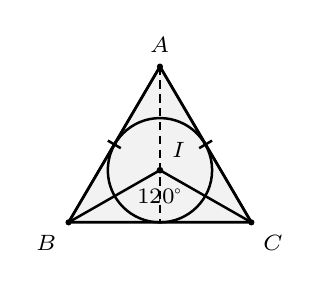
\begin{tikzpicture}[scale=0.86, every node/.style={font=\footnotesize, text=black}]
        \coordinate (B) at (-1.35,-0.85);
        \coordinate (C) at (1.35,-0.85);
        \coordinate (A) at (0,1.45);
        \coordinate (I) at (0,-0.08);
        \fill[gray!10] (A) -- (B) -- (C) -- cycle;
        \draw[black, line width=1.0pt] (A) -- (B) -- (C) -- cycle;
        \draw[black, line width=0.9pt] (I) circle (0.77cm);
        \draw[black, line width=0.9pt] (B) -- (I) -- (C);
        \draw[black, line width=0.8pt, densely dashed] (A) -- (0,-0.85);
        \draw[black, line width=0.8pt, tk1] (A) -- (B);
        \draw[black, line width=0.8pt, tk1] (A) -- (C);
        \fill[black] (A) circle (1.3pt) node[above=1.5pt] {$A$};
        \fill[black] (B) circle (1.3pt) node[below left=1pt] {$B$};
        \fill[black] (C) circle (1.3pt) node[below right=1pt] {$C$};
        \fill[black] (I) circle (1.4pt) node[above right=1pt] {$I$};
        \node at (0,-0.46) {$120^\circ$};
      \end{tikzpicture}
    \end{center}
    \vspace{-3pt}
    -- ដោយ $I$ ជាផ្ចិតរង្វង់ចារឹកក្នុង និង $\ang{B}=\ang{C}$ (មុំបាតត្រីកោណសមបាត) គេបាន៖\\
    \hspace*{0.25cm}$\ang{IBC} = \ang{BCI} = \dfrac{\ang{B}}{2} = \dfrac{\ang{C}}{2}$ (ហេតុផល \blank{0.7cm}) ។\\[2pt]
    -- ក្នុង $\tri{BIC}$ មាន $\ang{BIC}=120^\circ$ គេបាន៖\\
    \hspace*{0.25cm}$\ang{IBC} + \ang{BCI} = 180^\circ - 120^\circ = \blank{1.1cm}^\circ \Rightarrow 2\ang{IBC} = \blank{1.1cm}^\circ$\\
    \hspace*{0.25cm}$\Rightarrow \ang{IBC} = \blank{1.0cm}^\circ \Rightarrow \ang{B} = \ang{C} = 2 \times \blank{0.9cm}^\circ = \blank{1.0cm}^\circ$ ។\\[2pt]
    -- ត្រីកោណសមបាតមានមុំបាត $60^\circ$ ជាត្រីកោណ \textbf{\blank{2.1cm}}!
  \end{tcolorbox}
\end{minipage}%
\hfill
\begin{minipage}[t]{9.4cm}\vspace{0pt}
  \begin{tcolorbox}[
    enhanced, sharp corners, colback=white, colframe=black, equal height group=rowE4,
    boxrule=0.85pt, boxsep=2.2pt, top=3.5pt, bottom=3.5pt, left=5pt, right=5pt
  ]
    \textbf{៣.ខ ប្រតិបត្តិ (ទំ.២១២)៖ គណនាមុំ $\ang{BIC}$ ក្នុងត្រីកោណកែង}\\
    $\tri{ABC}$ ជាត្រីកោណកែងត្រង់កំពូល $A$ ($\ang{A}=90^\circ$) និង $I$ ជាផ្ចិតរង្វង់ចារឹកក្នុងនៃត្រីកោណនេះ ។ គណនាជាដឺក្រេនៃមុំ $\ang{BIC}$៖
    \begin{center}
      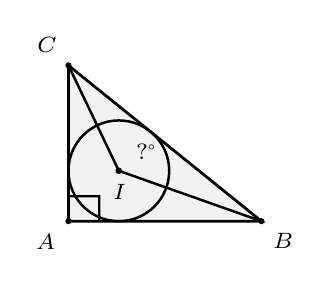
\begin{tikzpicture}[scale=0.86, every node/.style={font=\footnotesize, text=black}]
        \coordinate (A) at (-1.30,-0.85);
        \coordinate (B) at (1.55,-0.85);
        \coordinate (C) at (-1.30,1.45);
        \pgfmathsetmacro{\la}{veclen(2.85,2.30)}
        \pgfmathsetmacro{\rad}{(2.30+2.85-\la)/2}
        \coordinate (I) at (-1.30+\rad,-0.85+\rad);
        \fill[gray!10] (A) -- (B) -- (C) -- cycle;
        \draw[black, line width=1.0pt] (A) -- (B) -- (C) -- cycle;
        \rightbox[0.16]{C}{A}{B}
        \draw[black, line width=0.9pt] (I) circle (\rad cm);
        \draw[black, line width=0.9pt] (B) -- (I) -- (C);
        \fill[black] (A) circle (1.3pt) node[below left=1pt] {$A$};
        \fill[black] (B) circle (1.3pt) node[below right=1pt] {$B$};
        \fill[black] (C) circle (1.3pt) node[above left=1pt] {$C$};
        \fill[black] (I) circle (1.4pt) node[below=1.5pt] {$I$};
        \node at (-0.15,0.18) {$?^\circ$};
      \end{tikzpicture}
    \end{center}
    \vspace{-3pt}
    $1.$ ក្នុង $\tri{ABC}$ កែងត្រង់ $A$ គេមានផលបូកមុំស្រួចទាំងពីរ៖\\
    \hspace*{0.25cm}$\ang{B} + \ang{C} = \blank{1.2cm}^\circ$ ។\\[2.5pt]
    $2.$ ដោយ $BI$ និង $CI$ ជាកន្លះបន្ទាត់ពុះមុំក្នុងនៃ $\ang{B}$ និង $\ang{C}$៖\\
    \hspace*{0.25cm}$\ang{IBC} + \ang{ICB} = \dfrac{\ang{B}+\ang{C}}{2} = \dfrac{\blank{1.0cm}^\circ}{2} = \blank{1.1cm}^\circ$ ។\\[2.5pt]
    $3.$ ក្នុង $\tri{BIC}$៖ $\ang{BIC} = 180^\circ - (\ang{IBC}+\ang{ICB}) = \blank{1.3cm}^\circ$ ។\\[2.5pt]
    $\star$ \textbf{ឆ្លុះបញ្ចាំងទូទៅ៖} បើស្គាល់មុំ $\ang{A}$ នោះ $\ang{BIC} = 90^\circ + \dfrac{\blank{0.9cm}}{2}$!
  \end{tcolorbox}
\end{minipage}

\vspace{2pt}
% --- E5 Evaluate: Textbook Ex #7 (p.213) + Exit Check ---
\secbar{ផ្នែកទី៤ ៖ វាយតម្លៃលទ្ធផលសិក្សា \enbf{---} លំហាត់ទី៧ \enbf{(}ទំ\enbf{.}២១៣\enbf{)} និងសំណួរត្រួតពិនិត្យរហ័ស \enbf{(E5)}}{ធ្វើដោយឯករាជ្យ \en{10 min}}

\noindent
\begin{minipage}[t]{10.3cm}\vspace{0pt}
  \begin{tcolorbox}[
    enhanced, sharp corners, colback=white, colframe=black, equal height group=rowE5,
    boxrule=0.85pt, boxsep=2.2pt, top=3.5pt, bottom=3.5pt, left=5pt, right=5pt
  ]
    \textbf{៤.ក លំហាត់ទី៧ (ទំ.២១៣)៖ គណនាមុំក្នុងតារាងតាមរូប}\\
    \begin{minipage}[c]{5.0cm}
      សង្កេតរូបខាងស្ដាំ៖ ចំណុច $M$ មានចម្ងាយកែង $1\unit{cm}$ ស្មើគ្នាទៅជ្រុង $AB$ និង $BC$ ($\ang{ABM}=40^\circ$) ហើយ $\ang{ACM}=\ang{BCM}=15^\circ$ ។ ចូរបំពេញតារាងខាងក្រោម៖
    \end{minipage}%
    \hfill
    \begin{minipage}[c]{4.6cm}
      \centering
      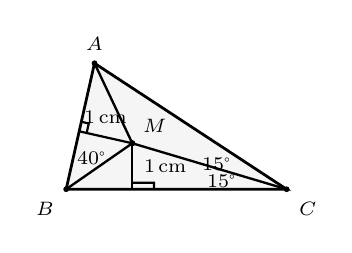
\begin{tikzpicture}[scale=0.80, every node/.style={font=\scriptsize, text=black}]
        \coordinate (B) at (-1.45,-0.75);
        \coordinate (C) at (2.05,-0.75);
        \coordinate (A) at (-1.00,1.25);
        \coordinate (M) at (-0.40,-0.02);
        \coordinate (P) at (-0.40,-0.75);
        \coordinate (R) at ($(A)!(M)!(B)$);
        \fill[gray!8] (A) -- (B) -- (C) -- cycle;
        \draw[black, line width=1.0pt] (A) -- (B) -- (C) -- cycle;
        \draw[black, line width=0.85pt] (A) -- (M) (B) -- (M) (C) -- (M);
        \draw[black, line width=0.8pt] (M) -- (P) node[midway, right=0.5pt] {$1\unit{cm}$};
        \draw[black, line width=0.8pt] (M) -- (R) node[midway, above=1pt] {$1\unit{cm}$};
        \rightbox[0.14]{M}{P}{C}
        \rightbox[0.14]{M}{R}{A}
        \fill[black] (A) circle (1.3pt) node[above=1pt] {$A$};
        \fill[black] (B) circle (1.3pt) node[below left=1pt] {$B$};
        \fill[black] (C) circle (1.3pt) node[below right=1pt] {$C$};
        \fill[black] (M) circle (1.4pt) node[above right=0.5pt] {$M$};
        \node at (-1.04,-0.25) {$40^\circ$};
        \node at (1.02,-0.62) {$15^\circ$};
        \node at (0.95,-0.36) {$15^\circ$};
      \end{tikzpicture}
    \end{minipage}\\[4pt]
    {\renewcommand{\arraystretch}{1.35}\footnotesize
    \begin{tabular}{|L{2.10cm}|C{1.45cm}|C{1.45cm}|C{1.45cm}|C{1.45cm}|}
      \hline
      \cellcolor{headgray}\textbf{មុំ} & \cellcolor{headgray}$\mathbf{\ang{MBC}}$ & \cellcolor{headgray}$\mathbf{\ang{BMC}}$ & \cellcolor{headgray}$\mathbf{\ang{CAM}}$ & \cellcolor{headgray}$\mathbf{\ang{AMC}}$ \\
      \hline
      \textbf{គិតជាដឺក្រេ} & \blank{1.05cm} & \blank{1.05cm} & \blank{1.05cm} & \blank{1.05cm} \\
      \hline
    \end{tabular}}\\[3pt]
    {\footnotesize $\blacktriangleright$ ហេតុអ្វី $M$ ជាផ្ចិតរង្វង់ចារឹកក្នុងនៃ $\tri{ABC}$? \blank{3.8cm}}
  \end{tcolorbox}
\end{minipage}%
\hfill
\begin{minipage}[t]{8.5cm}\vspace{0pt}
  \begin{tcolorbox}[
    enhanced, sharp corners, colback=white, colframe=black, equal height group=rowE5,
    boxrule=0.85pt, boxsep=2.2pt, top=3.5pt, bottom=3.5pt, left=5pt, right=5pt
  ]
    \textbf{៤.ខ សំណួរត្រួតពិនិត្យរហ័ស (\en{Exit Check})៖}\\
    ចូរគូសវង់ជុំវិញអក្សរនៃចម្លើយត្រឹមត្រូវតែមួយគត់៖\\[3.5pt]
    \textbf{សំណួរទី១៖} ផ្ចិតរង្វង់ចារឹកក្នុង $I$ នៃ $\tri{ABC}$ មានលក្ខណៈ៖\\
    \hspace*{0.15cm}\textbf{ក.} $IA = IB = IC$ \hspace{0.75cm}
    \textbf{ខ.} $IP = IQ = IR$ (កែងនឹងជ្រុង)\\
    \hspace*{0.15cm}\textbf{គ.} $IA = \frac{2}{3}AA'$ \hspace{0.92cm}
    \textbf{ឃ.} ឋិតលើមេដ្យាទ័រជានិច្ច\\[4.5pt]
    \textbf{សំណួរទី២ (បេសកកម្ម E1)៖} ដើម្បីគូសរង្វង់ចារឹកក្នុងត្រីកោណ តើត្រូវបើកដែកឈានតាមអង្កត់ណា?\\
    \hspace*{0.15cm}\textbf{ក.} អង្កត់ចំណោលកែង $IP$ \hspace{0.25cm}
    \textbf{ខ.} អង្កត់ទ្រេត $IB'$\\[4.5pt]
    \textbf{សំណួរទី៣៖} ចំពោះត្រីកោណមុំទាល តើផ្ចិតរង្វង់ចារឹកក្នុង $I$ ស្ថិតនៅត្រង់ណា?\\
    \hspace*{0.15cm}\textbf{ក.} ខាងក្នុងត្រីកោណជានិច្ច \hspace{0.18cm} \textbf{ខ.} ខាងក្រៅត្រីកោណ
  \end{tcolorbox}
\end{minipage}

\vspace{2pt}
% --- Step 5 Homework Box ---
\secbar{ផ្នែកទី៥ ៖ កិច្ចការផ្ទះ និងការរៀបចំមេរៀនបន្ទាប់ \enbf{(}សៀវភៅគោល ទំព័រ ២១៣\enbf{--}២១៤\enbf{)}}{ធ្វើនៅផ្ទះក្នុងសៀវភៅសរសេរ}

\begin{tcolorbox}[
  enhanced, sharp corners, colback=panelgray, colframe=black,
  boxrule=0.85pt, boxsep=2.5pt, top=3.5pt, bottom=3.5pt, left=6pt, right=6pt
]
  $1.$ \textbf{លំហាត់ទី៦ (ទំ.២១៣)៖} $\tri{ABC}$ ជាត្រីកោណកែងត្រង់ $A$ ។ រង្វង់ចារឹកក្នុងត្រីកោណនេះប៉ះទៅនឹងជ្រុងត្រីកោណត្រង់ចំណុច $P, Q$ និង $R$ ($I$ ជាផ្ចិតរង្វង់នេះ) ។ ប្រាប់ប្រភេទនៃចតុកោណ $APIQ$ ដោយបញ្ជាក់ហេតុផល ។\\[2.5pt]
  $2.$ \textbf{លំហាត់ទី១២ (ទំ.២១៤)៖} ក្នុង $\tri{ABC}$ កន្លះបន្ទាត់ពុះនៃមុំ $B$ និងមុំ $C$ ប្រសព្វគ្នាត្រង់ $I$ ។ ក្នុង $\tri{ADE}$ កន្លះបន្ទាត់ពុះនៃមុំ $D$ និងមុំ $E$ ប្រសព្វគ្នាត្រង់ $J$ ។ បង្ហាញថាចំណុច $A, I$ និង $J$ រត់ត្រង់ជួរគ្នា ។\\[2.5pt]
  $3.$ \textbf{កិច្ចការអានជាមុន៖} អានចំណុច \textbf{កន្លះបន្ទាត់ពុះក្រៅនិងកន្លះបន្ទាត់ពុះក្នុង} (ទំ.២១១\,\en{--}\,២១២៖ ផ្ចិតរង្វង់ចារឹកក្នុងមុំក្រៅត្រីកោណ $J$) ។
\end{tcolorbox}

\end{document}
